% ========== RESULTS SECTION ==========

% Fitted mu_EW values
The signal strength for \ac{EW} \VZy measured from the full fit is
%
\begin{equation*}
  \begin{split}
  \muEW &= 1.41 ^{+1.20}_{-1.14} \\
        &= 1.41 ^{+0.93}_{-0.90} \,(\text{stat.})
                 ^{+0.75}_{-0.70} \,(\text{syst.}),
  %\muEW &= 1.406 ^{+1.195}_{-1.142} \\
  %      &= 1.406 ^{+0.930}_{-0.901} \,(\text{stat.})
  %               ^{+0.750}_{-0.701} \,(\text{syst.}),
  \end{split}
\end{equation*}
% mu_EWK  1.40551 +1.19471 -1.1415
% mu_EWK  1.35899 +0.930069 -0.900662
%
and is compatible with the \ac{SM} expectation. Post-fit distributions in the
four regions are shown in Figure \ref{fig:vzy-results-postfit}, and the corresponding yields are given in Table \ref{tab:vzy-results-yields}.

% Post-fit yields
\begin{table}[!b]
  \centering
  \caption{
    Post-fit yields and uncertainties in each of the four regions included in
    the fit, and additionally for the final bin of the signal region. Yields
    are shown for each signal or background process individually, for the total
    signal+background yield, and for data.
}
  \begin{tabular}{p{2.5cm}ccccc}
    \midrule\midrule
    \multirow{2}{*}{Process} & \multicolumn{5}{c}{Yield} \\\cmidrule{2-6}
                             & \ac{BDT} \ac{CR} & $m_{jj}^\text{low}$ \ac{CR} &
                             $m_{jj}^\text{high}$ \ac{CR} & \ac{SR} & \ac{SR}$(\rarsig > 0.95)$ \\
    \midrule
    \ac{EW} \VZy  & $17 \pm 14    $&$ 1.4 \pm 1.5  $&$ 2.1 \pm 2.0  $&$ 31 \pm 25   $&$ 15   \pm 12     $\\
    \ac{QCD} \Zy  & $1360 \pm 40  $&$ 1320 \pm 50  $&$ 1970 \pm 60  $&$ 383 \pm 15  $&$ 112  \pm 7     $\\
    \tty          & $310 \pm 40   $&$ 206 \pm 25   $&$ 580 \pm 70   $&$ 50 \pm 6    $&$ 10.0 \pm 1.2  $\\
    Z+jets        & $157 \pm 23   $&$ 150 \pm 16   $&$ 270 \pm 60   $&$ 71 \pm 9    $&$ 18.4 \pm 2.2  $\\
    \ac{EW} \Zyjj & $17.6 \pm 0.8 $&$ 25.7 \pm 0.7 $&$ 27.8 \pm 0.7 $&$ 9.2 \pm 0.4 $&$ 3.34 \pm 0.16 $\\
    \WZjj         & $12.4 \pm 2.5 $&$ 12.1 \pm 2.4 $&$ 18 \pm 4     $&$ 4.2 \pm 0.8 $&$ 1.34 \pm 0.27 $\\\midrule
    Total         & $1884 \pm 28  $&$ 1718 \pm 31  $&$ 2870 \pm 40  $&$ 549 \pm 21  $&$ 159  \pm 11      $\\\midrule
    Data          & 1931         & 1697         & 2866         & 530         & 162           \\
    \midrule\midrule
  \end{tabular}
  \label{tab:vzy-results-yields}
\end{table}



% Post-fit distributions
\begin{figure}[tp]
  \centering
  \begin{subfigure}{.495\textwidth}
    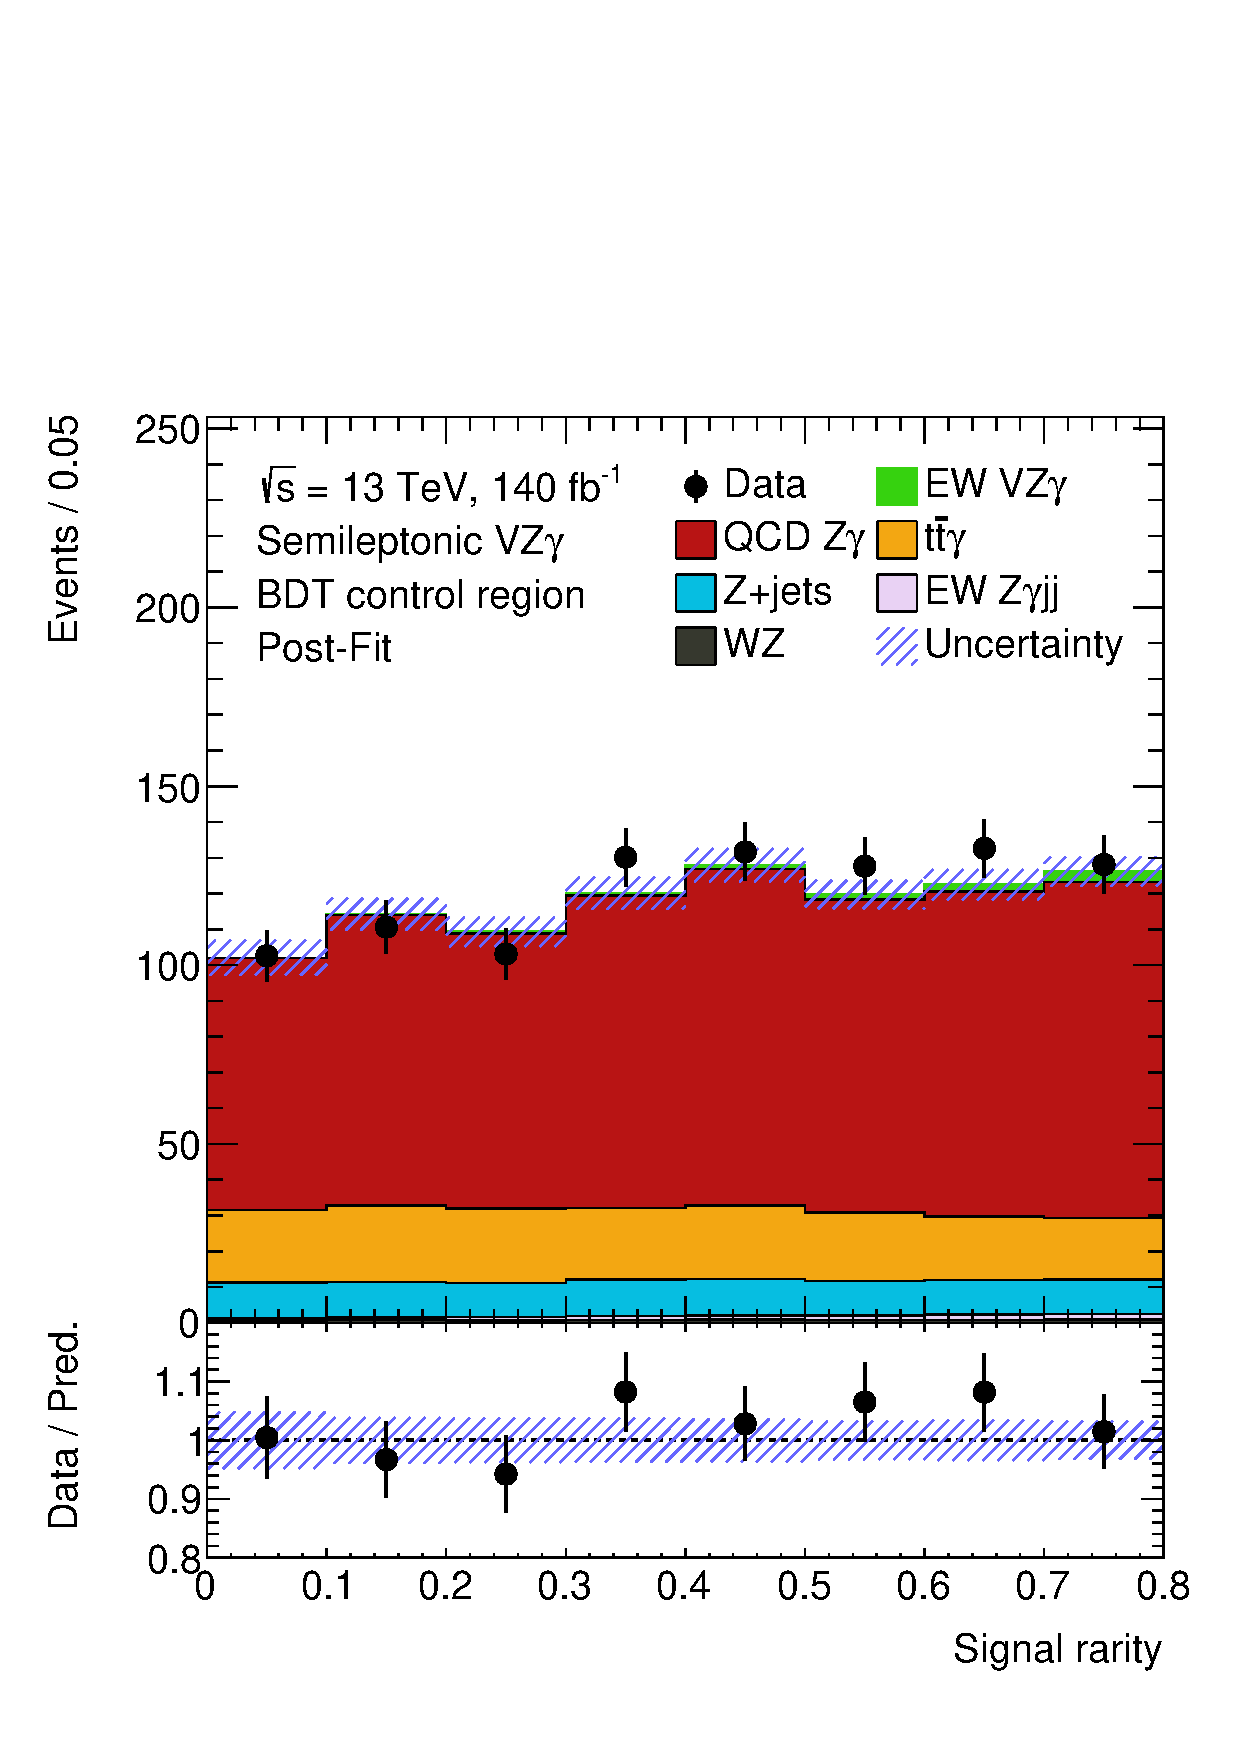
\includegraphics[width=\textwidth]{\resource{stack/CR_BDT_postFit.pdf}}
  \end{subfigure}
  \hfill
  \begin{subfigure}{.495\textwidth}
    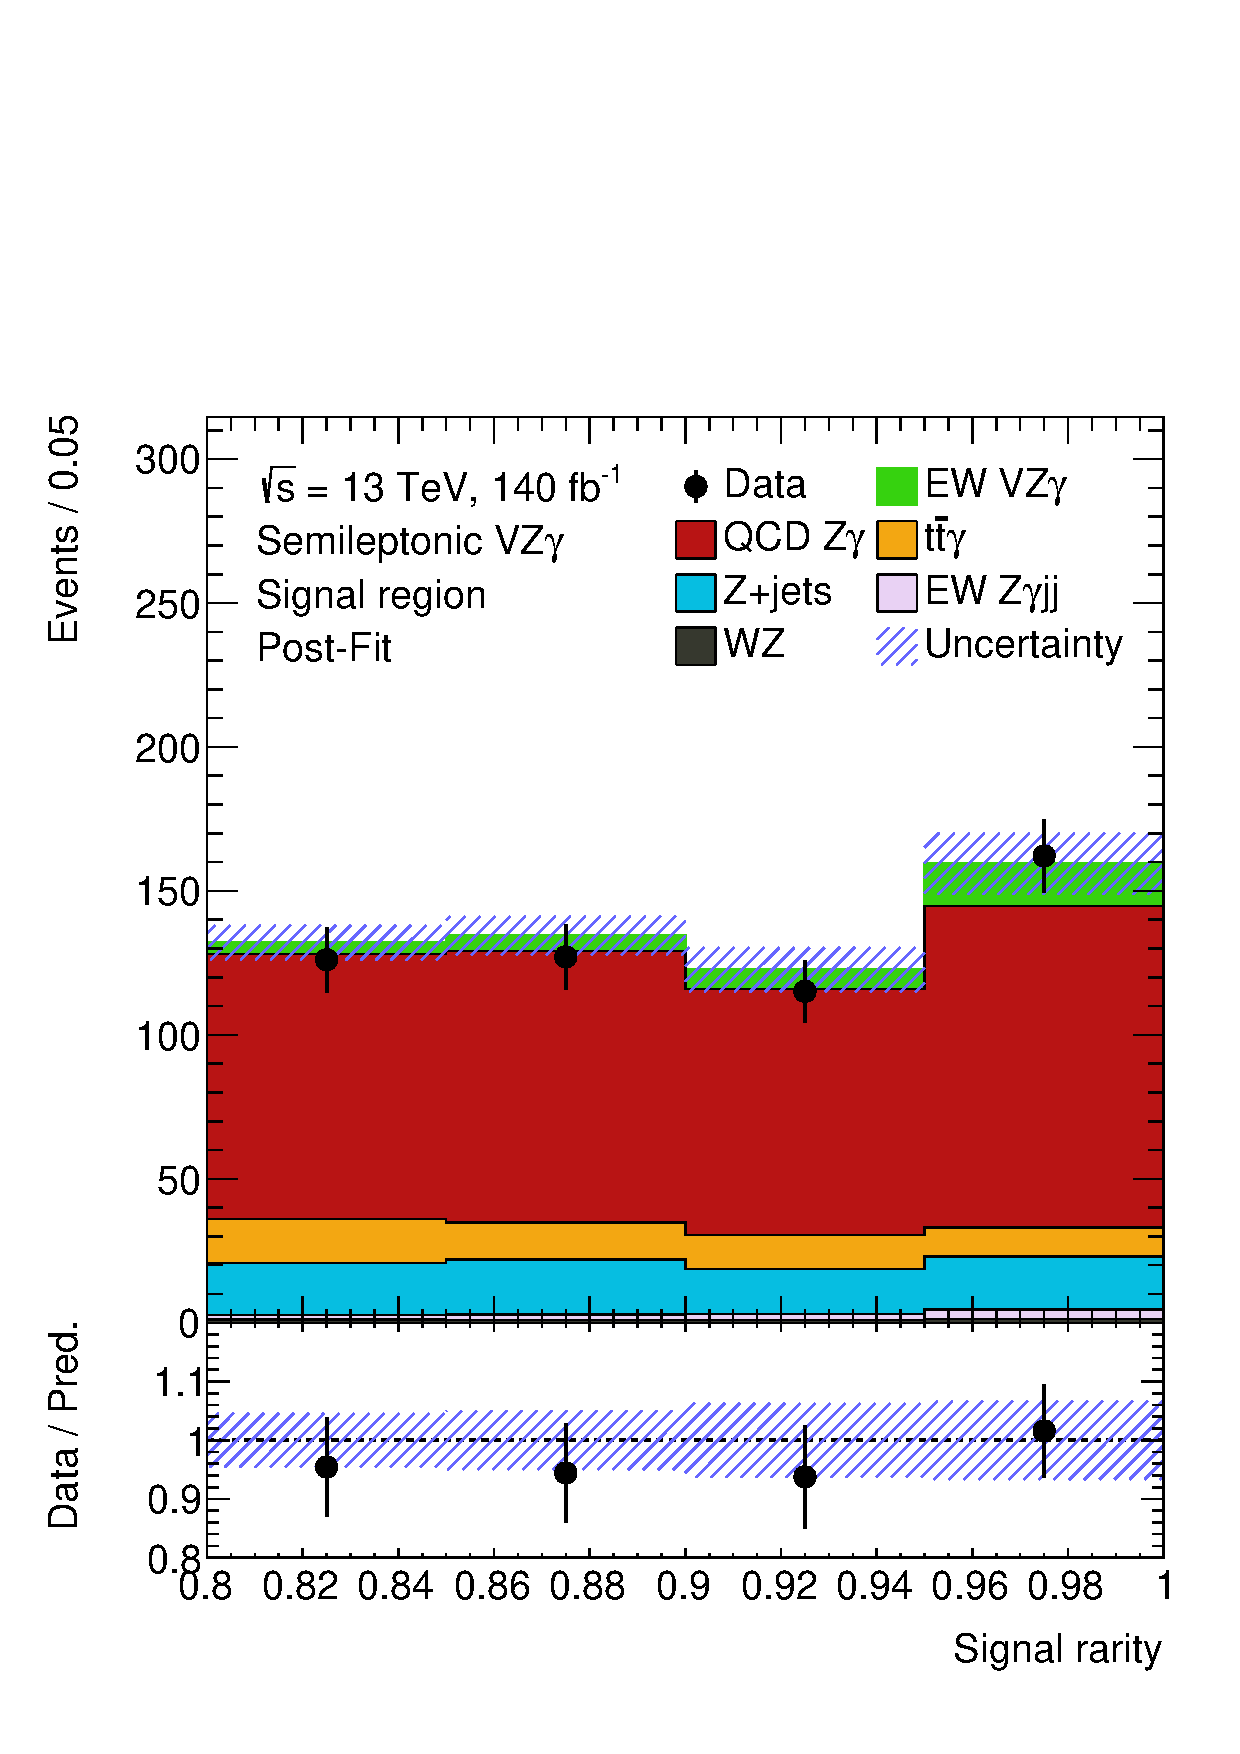
\includegraphics[width=\textwidth]{\resource{stack/SR_postFit.pdf}}
  \end{subfigure}
  \\[1em]%
  \begin{subfigure}{.495\textwidth}
    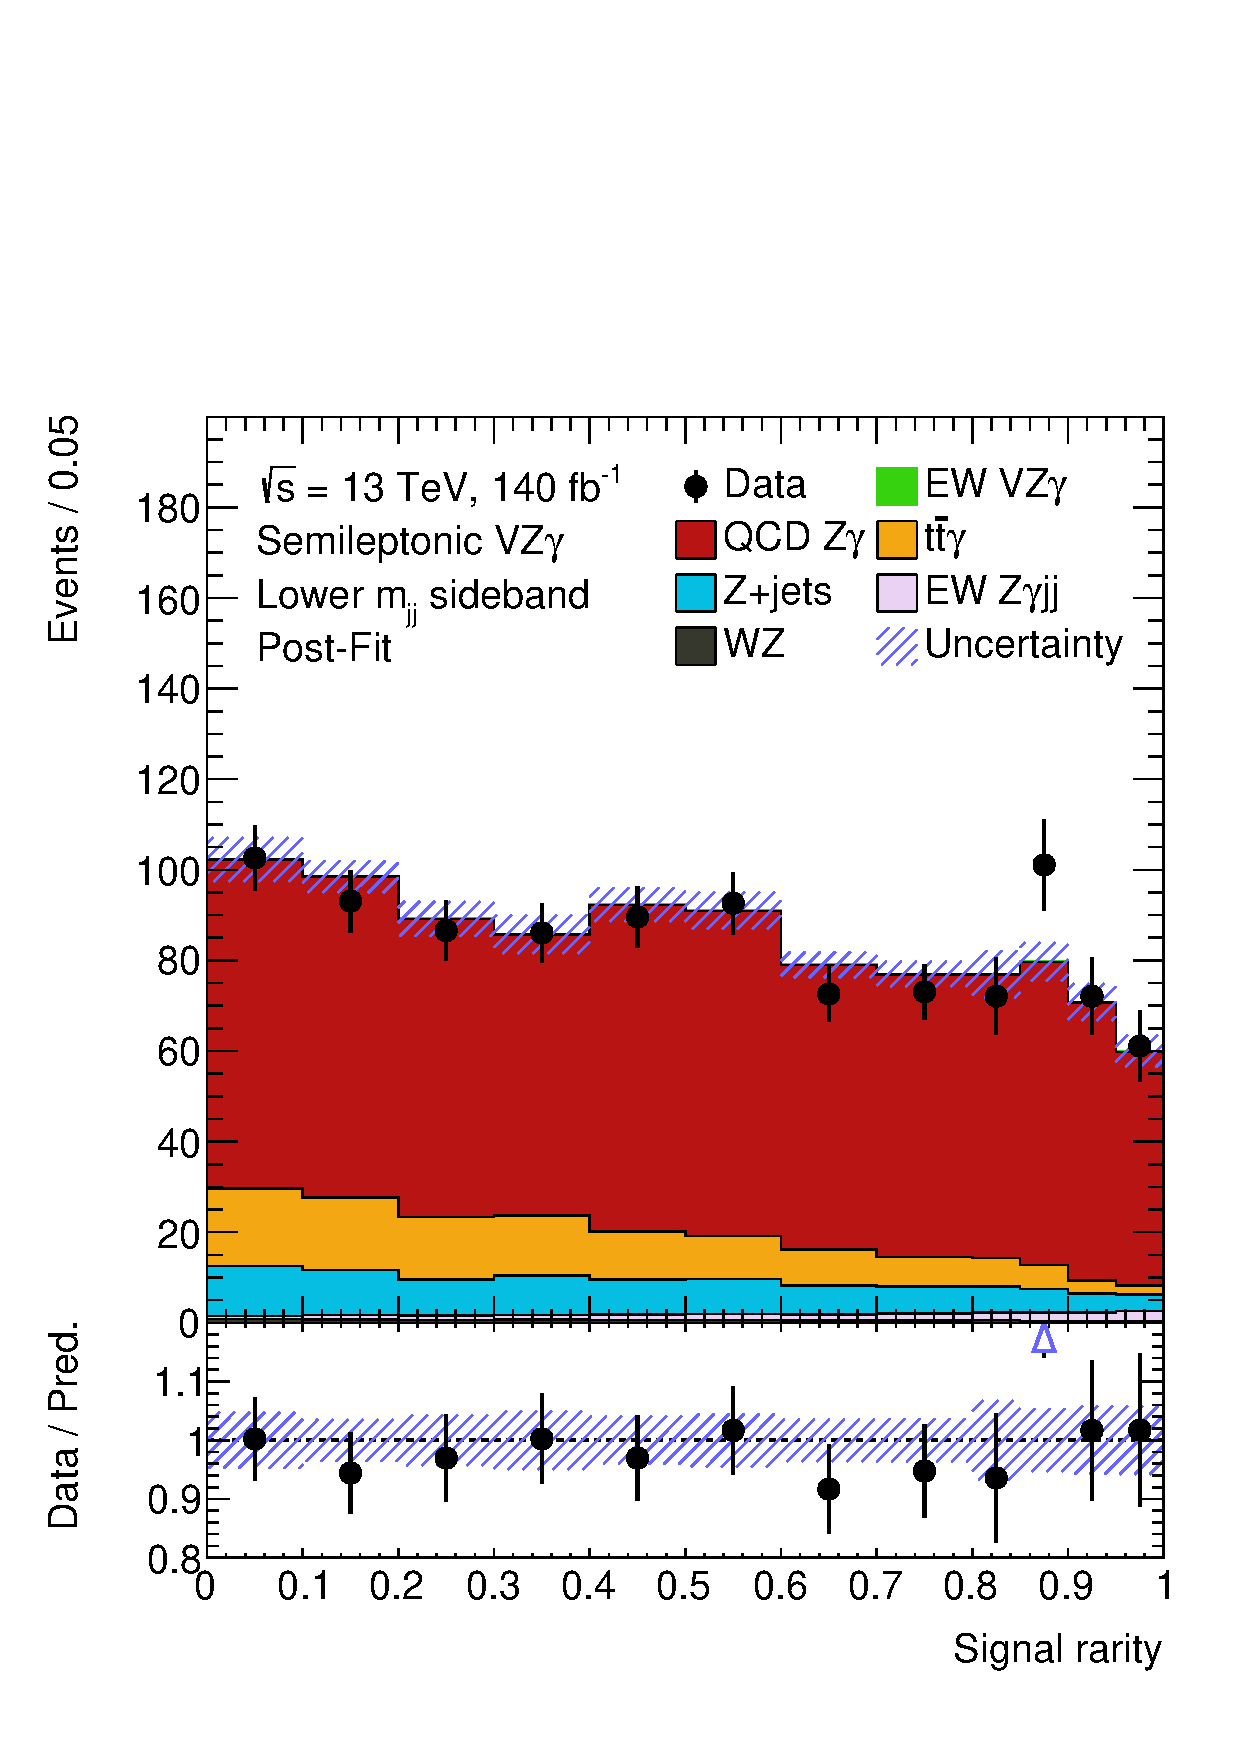
\includegraphics[width=\textwidth]{\resource{stack/CR_mjj_1_postFit.pdf}}
  \end{subfigure}
  \hfill
  \begin{subfigure}{.495\textwidth}
    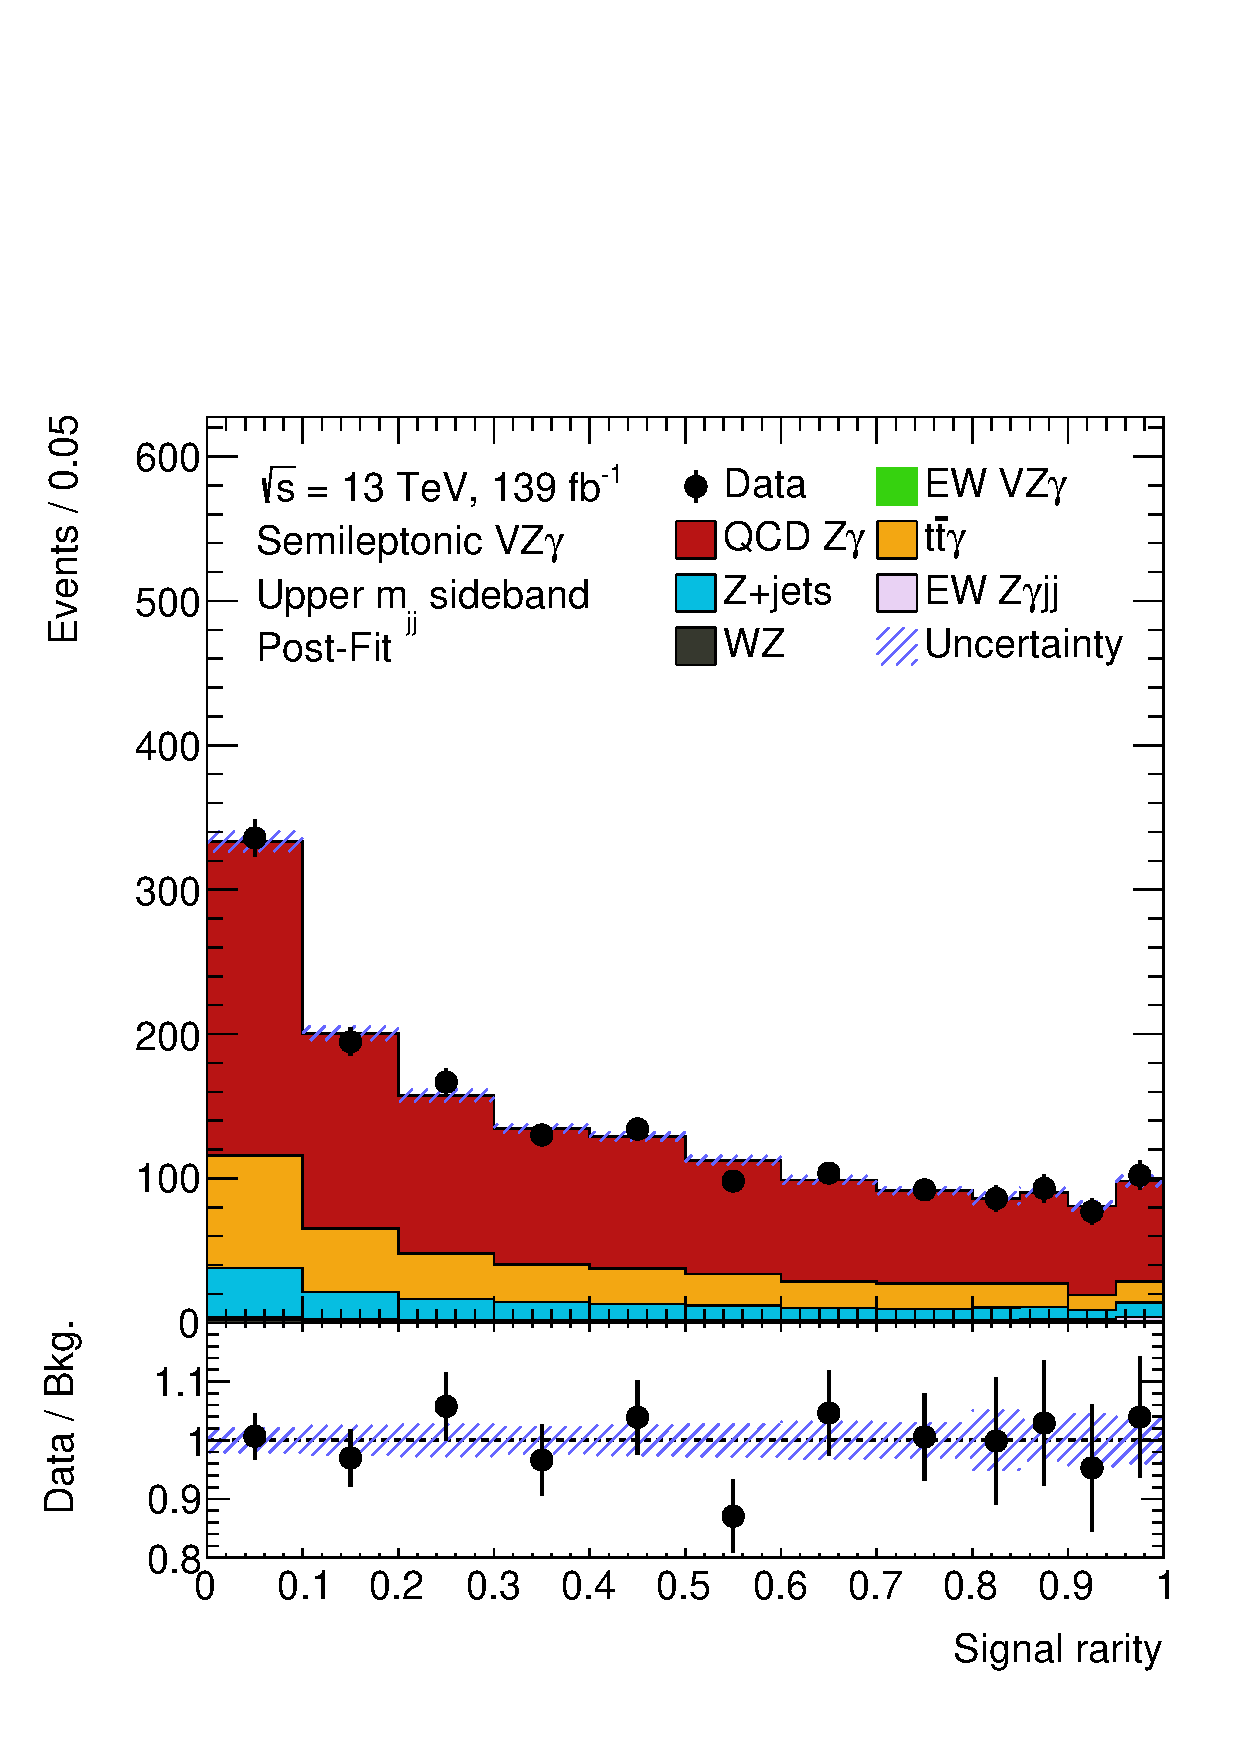
\includegraphics[width=\textwidth]{\resource{stack/CR_mjj_2_postFit.pdf}}
  \end{subfigure}
  \caption{
    Post-fit signal rarity distributions in each of the four regions used in the
    fit, as labelled. Uncertainty bands represent the combined uncertainties in
    each bin, with values constrained by the fit. Uncertainty on data is due to
    statistics. The lower sections of each plot give the ratio of the data to
    the total background estimate.
  }
  \label{fig:vzy-results-postfit}
\end{figure}

% Significance and limits
The observed significance of the signal process is 1.24 standard deviations,
compared with an expected significance of 1.40 standard deviations.  This does
not meet the threshold to provide evidence on the existence of the process.
Instead a 95\% confidence level upper limit is set on the rate of production for
signal events at 3.46 times the \ac{SM} expectation. This can be used to
constrain any new physics models that would enhance the cross-section for
triboson \VZy production.

%Injecting signal into the limit estimate: 1.000000
%Expected limit (median): 2.261164, worst case error: -0.026594
%Expected limit (-1 sig): 1.608560, worst case error: 0.028700
%Expected limit ( 1 sig): 3.203297, worst case error: -0.089267
%Expected limit (-2 sig): 1.188495, worst case error: 0.015355
%Expected limit ( 2 sig): 4.391544, worst case error: -0.135924
%Injected limit         : 3.044920, worst case error: 0.143740
%Observed limit         : 3.464933, worst case error: 0.234227
%Expected p-value mu = 1 (median)     : 0.186029, error: 0.000003
%Observed p-value (median)            : 0.107927, error: 0.000002
%Expected significance mu = 1 (median): 0.892623, error: -0.000011
%Observed significance (median)       : 1.237627, error: -0.000011

% Pulls and ranking (pulls necessary? don't understand them too well)
Statistical uncertainties make the largest contribution to the measurement, but
systematic uncertainties make a significant contribution. The largest systematic
contributions are shown in Figure \ref{fig:vzy-results-ranking}.
Pileup reweighting is the largest individual contribution, likely due to the
limited data statistics (see Section \ref{sec:vzy-projection}).
The second largest contribution is from jet flavour composition, and several more
of the largest uncertainties are \ac{MC} statistics uncertainties in signal
bins; as these uncertainties should be reducible, the effect of reducing some of
these systematic uncertainties is discussed in Section \ref{sec:vzy-projection}.

\begin{figure}[tb]
  \centering
  \includegraphics[width=.8\textwidth]{\resource{Ranking_mu_EWK.pdf}}
  \caption{
    Systematic uncertainties ranked by their post-fit impact on \muEW.
    Uncertainties labelled $\gamma$ represent \acs{MC} statistics uncertainties
    in the given bin.
  }
  \label{fig:vzy-results-ranking}
\end{figure}
% TODO more detail on what the ranking plot means
